\title{Umbau eines \textsc{Detroit Electric Cars}}
\team{%
    Yanick Frei,
		Marc Müller}

\client{Urs Jäger}

\coach{%
    Felix Jenni}

\fssummary{
    Ein altes Elektrofahrzeug aus dem Jahre 1918 wurde auf moderne Lithium-Ionen-Batterien umgerüstet. Zeitgleich wurde die Funktion des Fahrzeuges, insbesondere die Stufenschaltung, analysiert und bei Bedarf repariert.}

\fsgraphics{
    \begin{minipage}{0.47\textwidth}
        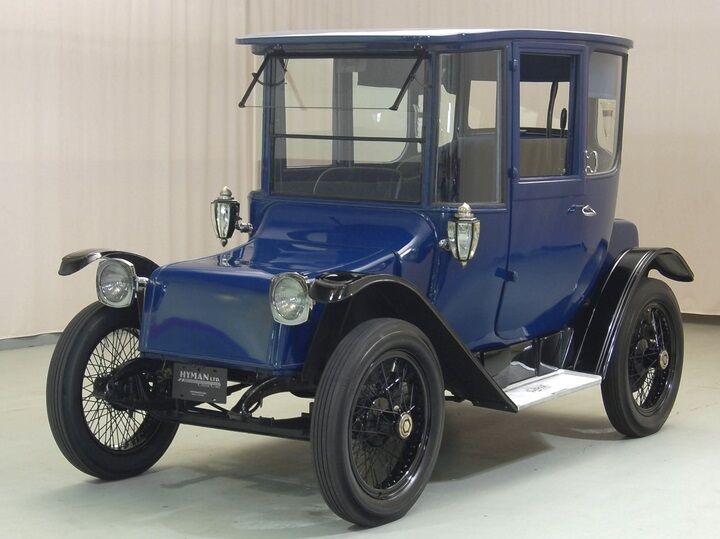
\includegraphics[height=54mm]{images/Detroit.jpg}
        \graphicscaption{Das Fahrzeug im aktuellen Zustand}
    \end{minipage}%
    \begin{minipage}{0.53\textwidth}
        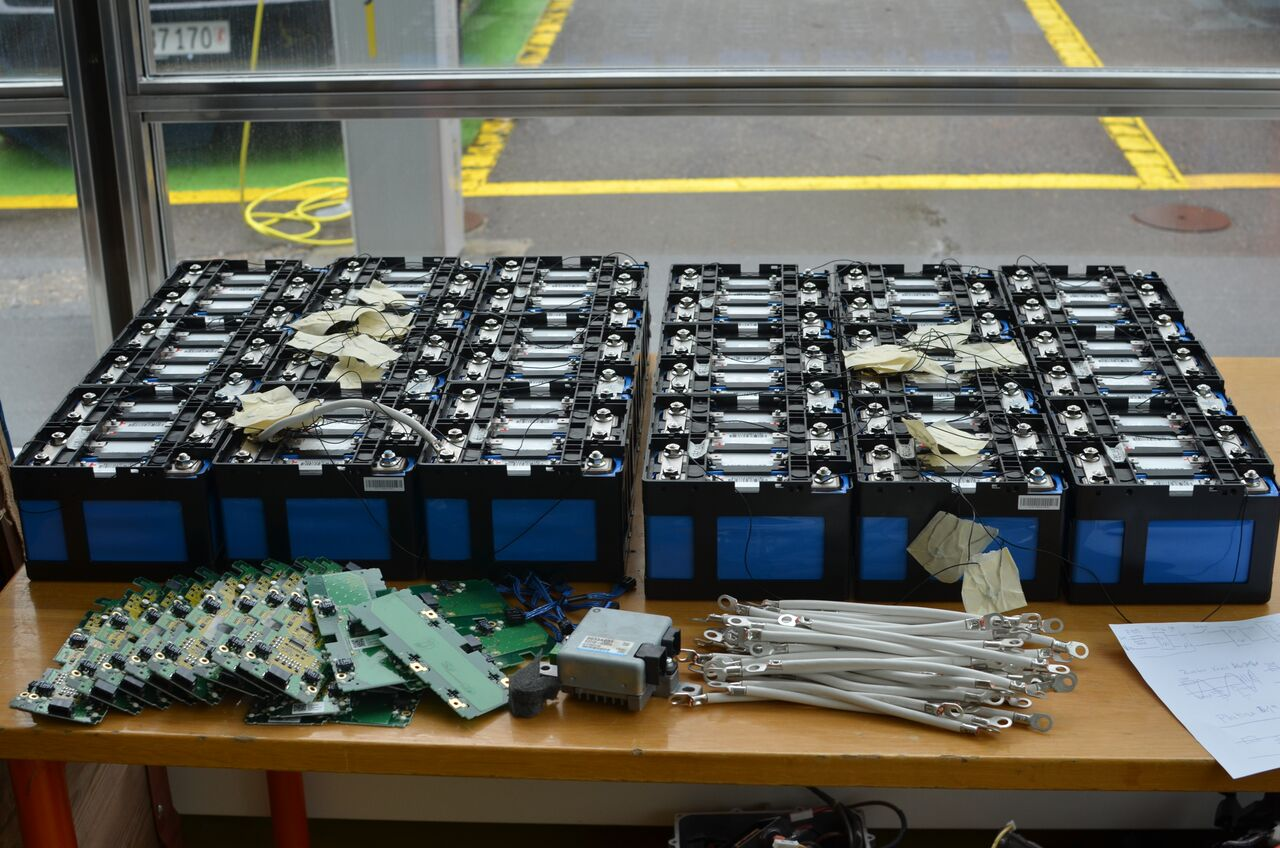
\includegraphics[height=54mm]{images/Batterie.jpg}
        \graphicscaption{Die Batterie vor dem Einbau}
    \end{minipage}
}

\fscontent{
    \section{Das Fahrzeug}
		Beim Fahrzeug handelt es sich um einen \textsc{Detroit Electric Car} aus dem Jahre 1918. Zu dieser Zeit waren Elektrofahrzeuge weit verbreitet und insbesondere bei Frauen beliebt, da das mühselige Anwerfen und die dreckigen Abgase bei Verbrennungsmotoren entfielen.
		
		Über mehrere Umwege kam das Fahrzeug zu einem Schweizer Sammler, jedoch in einem nicht fahrtüchtigen Zustand. Da die Batterie bereits einmal restauriert wurde und nicht mehr dem Original entsprach, wurden dort umfangreichere Anpassungen durchgeführt.
		
		\section{Der Antrieb}
		Angetrieben wird das Fahrzeug vom originalen Reihenschlussmotor von 1918. Reihenschlussmotoren besitzen dabei für Antriebe ein oftmals erwünschtes Verhalten, bei dem bei niedrigen Drehzahlen ein hohes Moment verfügbar ist, das bei hohen Drehzahlen stark abnimmt.
		
		Der Stufenschalter, welcher sich ebenfalls noch im Originalzustand befindet, regelt den Antrieb über Serie- und Parallelschaltung der beiden Batterien sowie Feldschwächung durch mehrere Erregerwicklungen. Widerstände werden nur kurzzeitig zum Anfahren benötigt.
		
		\section{Die Batterie}
		Im Fahrzeug wurden zwei identische Lithium-Ionen-Batterien verbaut. Lediglich die Zellen stammen aus einem Unfallfahrzeug, wohingegen weitere Komponenten wie das Batteriemanagementsystem oder die Ladegeräte extern eingekauft wurden.
		
		Das Batteriemanagementsystem überwacht zum einen den Zustand der Batterie in Bezug auf Sicherheit und Ladezustand, sorgt zum anderen aber auch dafür, dass alle Zellen stets auf dem selben Potential gehalten werden und sich dadurch keine aufschaukelnden Effekte einstellen können.
}

\infobox{Technische Daten}{%
    \small
    \setlength\tabcolsep{10pt}
    \begin{tabular}{lp{70mm}lp{55mm}}
    \bfseries Fahrzeug				& \\
    Hersteller:       				& \textsc{Detroit Electric Car Company} \\
    Baujahr:          				& 1918 (Annahme) \\
    Anzahl Fahrstufen:				& 5 Vorwärts; 1 Rückwärts \\
		Motortyp:									& Vierpoliger DC-Reihenschlussmotor \\
		Leistung:									& Ungefähr \SI{3.3}{\kilo\watt} (\SI{4.5} PS) \\
    Originaler Batterietyp:		& Bleibatterien \\
    Bremsen:          				& Trommelbremse (Hinterachse) \\
															& Bremsbacken (Motorschwungmasse) \\
		Reichweite:								& ca. \SI{100}{\kilo\meter} \\
															& \\
		\bfseries Batterie				& \\
		Technologie: 							& Lithium-Ionen \\
		Anzahl Batterien:					& Zwei \\
		Nennspannung:							& \SI{44.4}{\volt} \\
		Kapazität:								& \SI{150}{\ampere\hour} (Neuzustand) \\
															& \SI{70}{\ampere\hour} (Aktuell, 7 jährig) \\
		Ladeleistung:							& 2$\cdot$\SI{700}{\watt}
    \end{tabular}
}
